\chapter{Equilibrio del sólido rígido. Principio de los trabajos virtuales}	
\chaptermark{Equilibrio del sólido rígido}

\section{Equilibrio de los sistemas de partículas}

Las fuerzas externas que actúan son debidas al lugar que ocupa el sistema de partículas en el universo, son debidas a campos exteriores.

Las fuerzas interiores son las que se ejercen entre sí las partículas del sistema. Se supone que para estas fuerzas se cumple la tercera ley de Newton, la ley de acción y reacción:

$$ \overrightarrow{F}_{ij}=- \overrightarrow{F}_{ji} \ ; \qquad \sum_i \sum_j  \overrightarrow{F}_{ij}=0 $$

La condición de equilibrio es que la  $\overrightarrow{F}_{resultante}$ de todas las partículas del sistema sea cero. (Hemos llamado $\overrightarrow{F}_i' $ a las fuerzas de ligadura.)

$$\sum_j  \overrightarrow{F}_{ji} +  \overrightarrow{F}_i^{\ externas}+  \overrightarrow{F}_i'=\vec 0= \overrightarrow{F}_i+ \overrightarrow{F}_i'$$


Se han de satisfacer $N$ ecuaciones como la siguiente, una para cada una de las $N$ partículas que forman el sistema, con $\overrightarrow{F}_{ji} +  \overrightarrow{F}_i^{\ externas}=\overrightarrow{F}_i\ $. 

\section{Desplazamiento virtual}

Por \emph{desplazamiento virtual} infinitesimal de un sistema se entiende una variación de su configuración como resultado de cualquier cambio infinitesimal arbitrario $\ \boldsymbol{\var \vec r_i} \ $de las coordenadas de las partículas compatible con las fuerzas y ligaduras impuestas al sistema en un instante dado $ t $. Es un cambio infinitesimal del sistema de coordenadas que ocurre mientras el tiempo se mantiene fijo. Se le llama \emph{virtual} en vez de real dado que ningún desplazamiento real puede ocurrir sin que el tiempo avance.



En la mecánica analítica el concepto de desplazamiento virtual solo es significativo cuando se analiza un sistema físico sujeto a ligaduras que restringen su movimiento. El desplazamiento virtual $\var r$  es un caso especial de desplazamiento infinitesimal (normalmente denotado por $\dd r$) que se refiere a un cambio infinitesimal en las coordenadas de posición de un sistema de manera que las ligaduras se satisfacen.

\begin{multicols}{2}
Por ejemplo, una tiza sobre una mesa. En ambas posiciones hay equilibrio.

\begin{figure}[H]
	\centering
	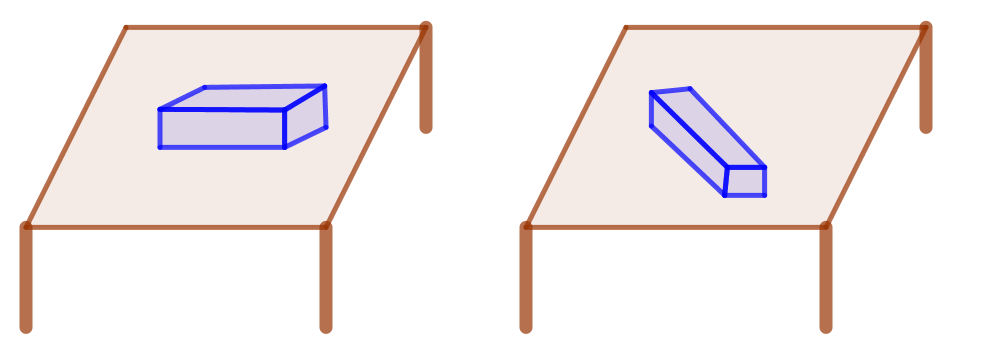
\includegraphics[width=.4\textwidth]{imagenes/imagenes06/T06IM01.png}
\end{figure}
\end{multicols}

En \emph{estática} el tiempo no va a intervenir como una magnitud fundamental para el estudio.

La condición de equilibrio es independiente del tiempo real, es como si congelásemos el tiempo. Introduciremos como parámetro el \emph{tiempo virtual}.

\section{Ligaduras sin rozamiento}

Las ligaduras se llaman sin rozamiento si el trabajo realizado por esas fuerzas de ligadura es cero.  (Una fuerza de rozamiento no es una fuerza de ligadura de rozamiento.)


Si el sistema se encuentra sometido exclusivamente a enlaces ideales (sin rozamiento), las fuerzas de enlace son ortogonales al propio enlace material, y como los desplazamientos $\var r_i$ deben ser compatibles con los enlaces, serán vectores ortogonales a las fuerzas de ligadura, por lo que no realizarán trabajo.	

Fuerzas de ligadura sin rozamiento $\ \bot \ $ a los desplazamientos. (*)

\section{Principio de los trabajos virtuales}

Solo es aplicable a fuerzas aplicadas y fuerzas de ligadura sin rozamiento.

\begin{miparrafo}
\emph{Para que un sistema de puntos materiales sujeto a `enlaces sin rozamiento' esté en equilibrio bajo la acción de un conjunto de fuerzas solicitantes es necesario y suficiente que sea nula la suma de los trabajos virtuales elementales efectuados por las fuerzas solicitantes para cualquier desplazamiento de dicho sistema efectuado a partir de una posición de equilibrio.}
\end{miparrafo}

$\displaystyle \sum_i (\vec F_i+\vec F_i')\cdot \var \vec r_i=
\sum_i \vec F_i\cdot \var \vec r_i +
\cancelto{0,\ (*)}{\sum_i \vec F_i'\cdot \var \vec r_i} \to 
 $
 
 \begin{equation}
 \subrayado{\boxed{\ \boldsymbol{\sum_i \vec F_i\cdot \var \vec r_i}=0 \ }}	
 \end{equation}


El trabajo total efectuado por las fuerzas aplicadas o solicitantes es nulo.

$ \displaystyle \sum_i  (\ F_{x_i}\cdot \var  x_i + F_{y_i}\cdot \var  y_i +F_{z_i}\cdot \var  z_i \ )=0 $

\begin{multicols}{2}
La figura muestra una aplicación sencilla de este principio a un sistema de una sola partícula y una sola fuerza aplicada, el peso.
El punto $B$ no es un punto de equilibrio, pues en el desplazamiento virtual indicado en la figura el peso realiza trabajo. El punto $A$ si es de equilibrio, pues cualquier desplazamiento virtual es perpendicular al peso y, por tanto, el peso no realiza trabajo.
\begin{figure}[H]
	\centering
	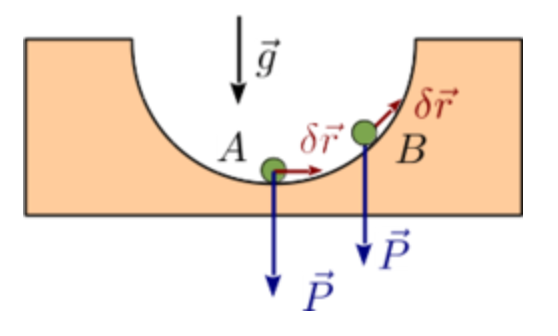
\includegraphics[width=.4\textwidth]{imagenes/imagenes06/T06IM02.png}
\end{figure}
\end{multicols}

\section{Sólido rígido}
Un cuerpo \emph{sólido rígido} es aquel cuerpo que está constituido por un sistema de partículas tal que las distancias entre las distintas partículas permanecen inalteradas y constantes en el tiempo.

En la naturaleza no existen sólidos rígidos, los cuerpos están formados por átomos y moléculas que vibran en sus posiciones de equilibrio. El sólido rígido es una idealización (abstracción de la realidad), es un conjunto de puntos del espacio que se mueven de tal manera que no se alteran las distancias entre ellos, sea cual sea la fuerza actuante.

\begin{figure}[H]
	\centering
	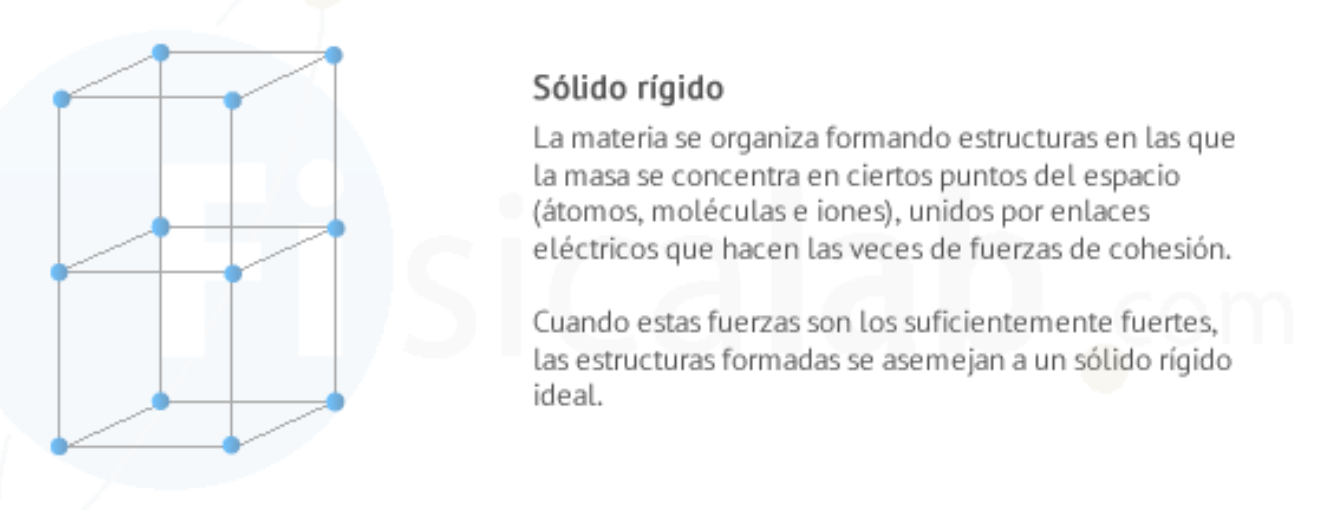
\includegraphics[width=1\textwidth]{imagenes/imagenes06/T06IM03.png}
\end{figure}

La mecánica de un cuerpo rígido es aquella que estudia el movimiento y equilibrio de sólidos materiales ignorando sus deformaciones. Se trata, por tanto, de un modelo matemático útil para estudiar una parte de la mecánica de sólidos, ya que todos los sólidos reales son deformables. 

\section{Equilibrio del solido rígido libre}

\begin{multicols}{2}
Para determinar la posición de un cuerpo rígido debemos dar las coordenadas de un punto, su centro de masas o centro de gravedad por ejemplo y de un eje del cuerpo. La posición del eje puede determinarse dando tres ángulos, los ángulos directores.

\begin{figure}[H]
	\centering
	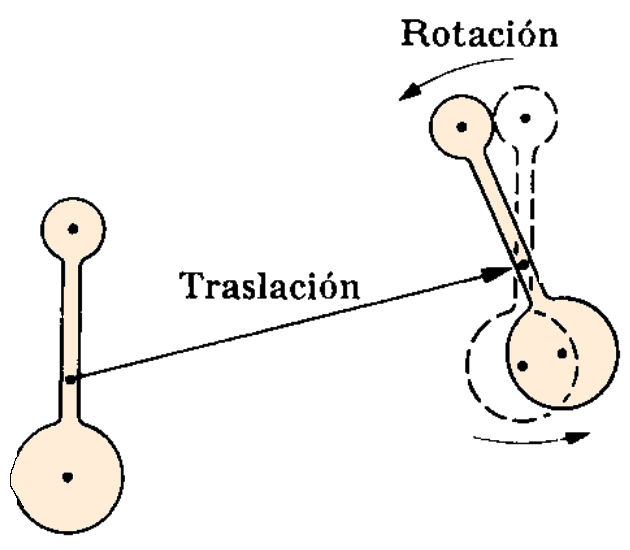
\includegraphics[width=.4\textwidth]{imagenes/imagenes06/T06IM04.png}
\end{figure}
\end{multicols}

La posición de un cuerpo rígido depende de $6$ parámetros, tiene $6$  grados de libertad: $3$ coordenadas del punto y $3$ ángulos directores del eje. De estos $6$ parámetros o grados de libertad, $3$ corresponden al movimiento y otros $3$ a la rotación.

Utilizaremos el método o principio de los trabajos virtuales: $\displaystyle \sum_i \vec F_i \cdot \var \vec r_i=0$

Non inventamos un tiempo virtual: $\displaystyle \vec v_i=\dv{\vec r_i}{t} \ \to \ \fdv{\vec r_i}{t}=\vec v_i$

Dividienndo por el tiempo virtual (sin existencia real) la ecuación de los trabajos virtuales:

\begin{equation}
 \sum_i\vec F_i\cdot \vec v_i=0	
\end{equation}

Ecuación que recibe el nombre de \emph{principio de las potencias virtuales.}

Particularizando al sólido rígido, se verifica que dadas 2 partículas $i$, $j$ de éste se cumple que (la demostración se verá en capítulos futuros):

$\vec v_i=\vec v+\vec w \times \vec r_i\ , \quad$
con $\vec v$ y $\vec w$, en principio, dos velocidades arbitrarias.
Sustituyendo en la ecuación de las potencias virtuales:

$\displaystyle \sum_i \vec F_i \cdot (\vec v+\vec w \times \vec r_i)=0 \ \to \ \vec v \cdot \sum_i \vec F_i + \sum_i \vec F_i \cdot (\vec \omega \times \vec r_i)=0 \quad (**)$

Como aparece un \emph{producto mixto} en el segundo término de la ecuación anterior y recordando sus propiedades (al cambiar dos filas de un determinante, éste no varía):

$\left| \begin{matrix} F_{i_x}&F_{i_y}&F_{i_z} \\ \omega_x&\omega_y&\omega_z \\ x_i&y_i&z_i \end{matrix} \right| \ = \ \left| \begin{matrix}\omega_x&\omega_y&\omega_z \\ x_i&y_i&z_i \\ F_{i_x}&F_{i_y}&F_{i_z} \end{matrix} \right|$

Por lo que: $\displaystyle \sum \vec F_i \cdot (\vec \omega \times \vec r_i) = \sum_i \vec \omega \cdot (\vec r_i \times \vec F_i) = \vec \omega \cdot \sum_i (\vec r_i \times \vec F_i) $

Por lo que la ecuación $(**)$ queda como:$\quad \vec v \cdot \sum_i \vec F_i +\vec \omega \cdot \sum_i (\vec r_i \times \vec F_i)=0$

Puesto que, como hemos dicho anteriormente, $\vec v$ y $\vec w$ son dos velocidades arbitrarias, necesariamente los coeficientes que las multiplican en la ecuación anterior deben ser cero:

\begin{eqnarray}
\sum_i \vec F_i&=&\vec 0 \\
\sum \vec r_i \times \vec F_i&=&\vec 0
\end{eqnarray} 

La \emph{suma de fuerzas solicitantes igual a cero} y la \emph{suma de los momentos de las fuerzas solicitantes igual a cero} son las dos ecuaciones vectoriales ($3+3$ ecuaciones escalares) del equilibrio del sólido rígido.

Las $6$ ecuaciones escalares del equilibrio del sólido rígido son:

\begin{eqnarray*}
\sum_i F_{i_x}=0 &\quad \quad \quad & \sum_i (y_i F_{z_i}-F_{y_i}z_i)=0 \nonumber \\
\sum_i F_{i_y}=0 &\quad \quad \quad & \sum_i (z_i F_{x_i}-F_{z_i}x_i)=0 \nonumber \\
\sum_i F_{i_z}=0 &\quad \quad \quad & \sum_i (x_i F_{y_i}-F_{x_i}y_i)=0 \nonumber  	
\end{eqnarray*}

Como ejemplo veremos el equilibrio del \emph{sólido plano}, que no existe en la realidad pero con ello queremos decir que el movimiento transcurre en un plano, supongamos el $XY$ 

Harán falta tres ecuaciones: 

\hspace{2cm} $\displaystyle \sum_i F_{x_i}=0;\ \ \sum_i F_{i_y}=0; \ \ \sum_i (x_iF_{y_i}-F_{x_i}y_i)=0$
 

\section{Equilibrio del sólido plano}


Supongamos una varilla rígida de masa $m$ unida a dos puntos $\mathcal O$ y $C$ por dos resortes  con una fuerza atractiva proporcional a la distancia. Tenemos que averiguar la posición de equilibrio, que sabemos quedará determinada por 3 parámetros. La longitud $2L$ de la barra es un dato.

Plano de movimiento $XY \quad \to \quad \begin{cases}
 \sum_i F_{x_i}=0 \\ \sum_i F_{i_y}=0 \\ \sum_i (x_iF_{y_i}-F_{x_i}y_i)=0	 \end{cases}$
 
 La única componente del momento de las fuerzas aplicadas o solicitantes que es perpendicular al plano $XY$ de movimiento es $M_z$, en la dirección $\vec k$.
 
 \begin{figure}[H]
	\centering
	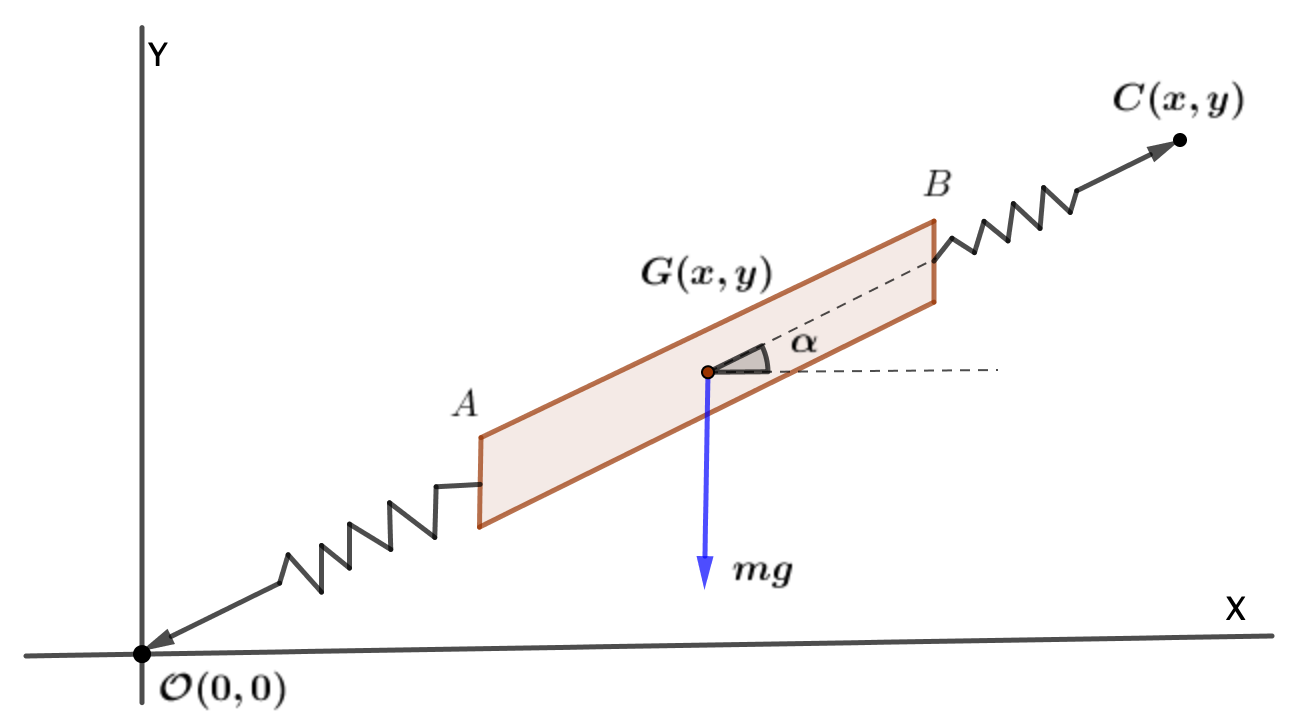
\includegraphics[width=.7\textwidth]{imagenes/imagenes06/T06IM05.png}
\end{figure}
 
 
 $\vec F_A=K\ \overrightarrow{AO}=K\ (-\vec i x_A-\vec j y_A)$
 
 $\vec F_B=K\ \overrightarrow{BC}=k\ (\vec i (x_C-x_B)+\vec j (y_C-y_B))$
 
 $\vec F_G=-\vec j\ mg$
 
 $x_A=\overline x-L\cos \alpha \qquad x_B=\overline x+L\cos \alpha$
 
  $y_A=\overline y-L\cos \alpha \qquad y_B=\overline y+L\cos \alpha$
 
  
$ \sum_i F_{x_i}=0 \ \to$ 
 
$\qquad k(-x_A+x_c-x_B)=0 $ 
    
$\sum_i F_{y_i}=0 \ \to$
 
$\qquad k(-y_A+y_c-y_B)-mg=0$
  
$ \sum_i(x_iF_{y_i}-y_iF_{x_i})=0 \ \to$

$\qquad  -x_AKy_A+y_Akx_A+x_Bk(y_C-y_B)-y_Bk(x_c-x_B)-\overline x mg=0 $
  
 Sustituyendo los valores de $x_A,\ x_B,\ y_A,\ y_B$ en función de $\overline x,\ \overline y,\ \alpha$ se obtiene un sistema de tres ecuaciones con las tres incógnitas, $\overline x,\ \overline y,\ \alpha$ , que determinan la posición de equilibrio del sólido plano.
 
 \section{Equilibrio del sólido rígido sometido a enlaces}
 \subsection{Equilibrio del sólido rígido que tiene un punto fijo}

\vspace{-5mm} %*********************************** 
  \begin{figure}[H]
	\centering
	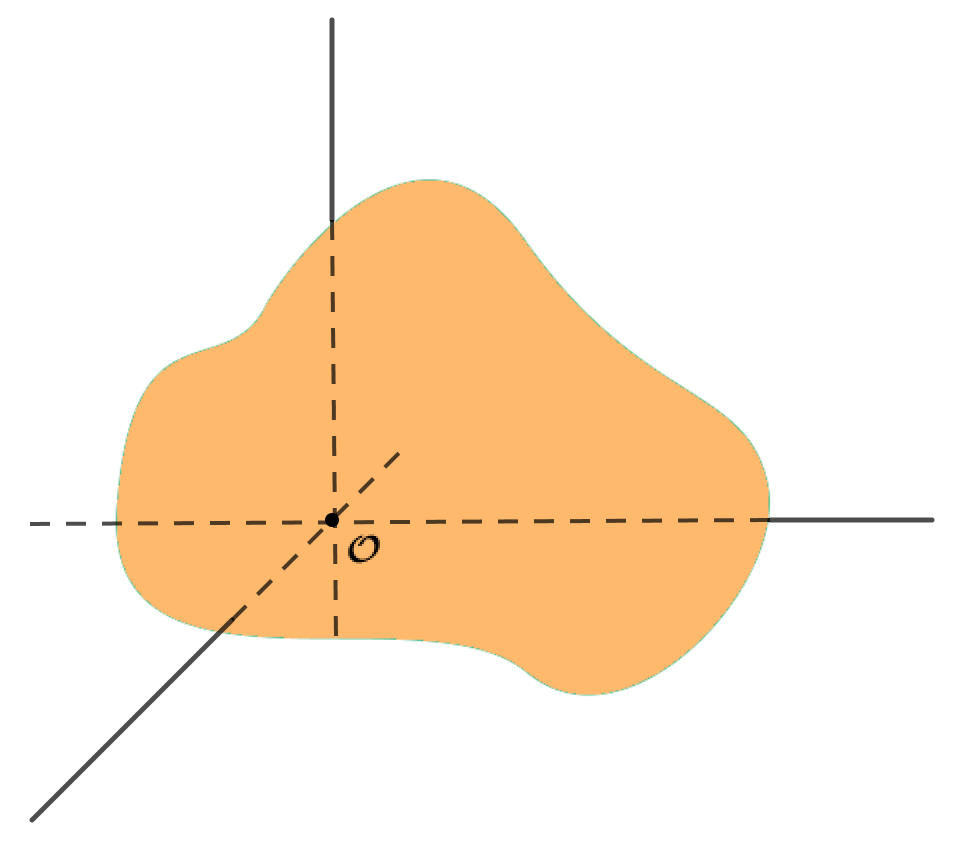
\includegraphics[width=.6\textwidth]{imagenes/imagenes06/T06IM06.png}
\end{figure}
 
 $$\vec v \cdot \displaystyle \sum_i \vec F_i + \vec w\cdot \sum_i(\vec r_i \times \vec F_i)=0$$
 
 Elegimos como velocidad $\vec v$ la que tiene el punto ligado $\mathcal O \ \to \ \vec v=0;\ \ \vec v_i=\vec \omega \times \vec r_i \to $ condiciones de equilibrio: $\displaystyle \sum_i (\vec r_i \times \vec F_i)=\vec 0$
 
 Luego, $\quad \begin{cases} 
 \ \displaystyle \sum_i (y_iF_{z_i}-z_iF_{y_i}=0\\
  \ \displaystyle \sum_i (z_iF_{x_i}-x_iF_{z_i}=0\\
   \ \displaystyle \sum_i (x_iF_{y_i}-y_iF_{x_i}=0\\	
 \end{cases}$


  \subsection{Equilibrio del sólido rígido que tiene dos puntos fijos}
 
\vspace{-5mm} %***********************************  
   \begin{figure}[H]
	\centering
	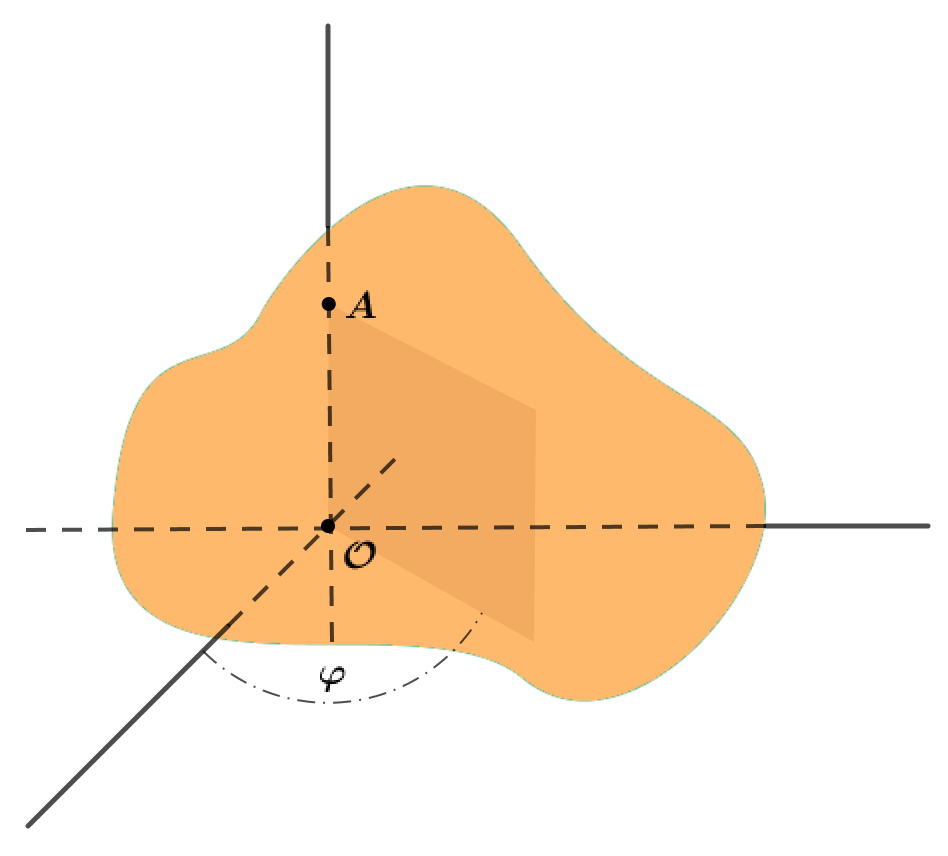
\includegraphics[width=.6\textwidth]{imagenes/imagenes06/T06IM07.png}
\end{figure}

Por el mismo razonamiento que en el caso anterior, la condición de equilibrio es $\displaystyle \sum_i \vec r_i \times \vec F_i=\vec 0$. En el plano $X-Y$ queda la tercera componente por ser perpendicular al eje giro  $\mathcal O A$:

$$\displaystyle \sum_i (x_iF_{y_i}-y_iF_{x_i})=0$$
 
 
 \section{Problemas}
 
 \begin{prob}
 	Usando el principio de los trabajos virtuales, determinar la posición de equilibrio de una partícula de masa $m$, móvil sobre la circunferencia $x^2+y^2=r^2$ y repelida por un punto fijo $C$, de coordenadas $(r/2,r/2)$, proporcionalmente a la distancia.
 \end{prob}

\begin{multicols}{2}
Principio trabajos virtuales:

$\displaystyle \sum_i \ \vec F_i \cdot \var \vec r_i = 0 \to$

$\displaystyle F_x \var x + F_y \var y =0$

$F_C=kd=$

$=k[(x-r/2)^2+(y-r_2)^2]^{1/2}$
\begin{figure}[H]
	\centering
	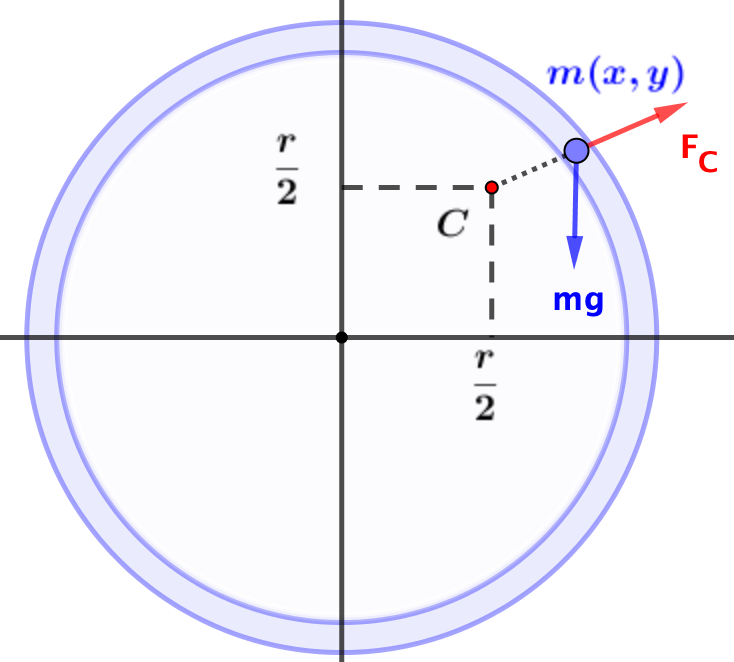
\includegraphics[width=.35\textwidth]{imagenes/imagenes06/T06IM08.png}
\end{figure}	
\end{multicols}

\vspace{-5mm} %*******************************************
$F_{C_x}=k(x-r/2)\ \vec i;\ \ F_{C_y}=k(y-r/2)\ \vec j;$
$\quad m\vec g=mg\ \vec j$ 

$F_x=k(x-r/2);\quad F_y=k(y-r/2)-mg$

Ppio. trabajos virtuales: $k(x-r/2)\ \var v+[k(y-r(2)-mg]\ \var y$

Ligadura: $x^2+y^2=r^2 \to \begin{cases} \ y=(r^2-x^2)^{1/2} \\ 2x\var x+2y \var  y=0 \to \var y=-\dfrac x{(x^2-r^2)^{1/2}} \var x \end{cases}$

Llevando estas relaciones al principio de los trabajos virtuales se obtiene: $f(x)\var x=0$, como $\var x \neq 0$ (el principio se enuncia para desplazamientos virtuales arbitrarios) $\to$ necesariamente, ha de ser $f(x)=0 \to x=x_{eq} \to (x^2+y^2=r^2) \to y=y_{eq}$.

\rightline{\textsf{\textcolor{DarkBlue}{--- Inacabado ---}}}

\begin{prob}
\begin{multicols}{2}
En la figura se observa una barra de peso $P$ y longitud $L$ que está oblgada a deslizar sus extremos entre dos rectas verticales entre sí. Hallar los puntos de equilibrio si es el peso que pende de la polea $\mathcal O$.
\begin{figure}[H]
	\centering
	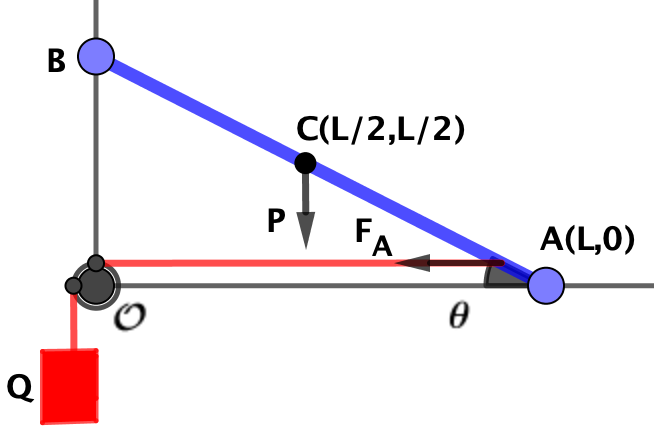
\includegraphics[width=.4\textwidth]{imagenes/imagenes06/T06IM09.png}
\end{figure}
\end{multicols}	
\end{prob}

$\vec F_A=-Q \vec i; \ \ \vec F_C=-P \vec j; \qquad \vec r_A=x_A \vec i = L\cos \theta \vec i; \ \  \vec r_C=\frac L 2 \cos \theta \vec i + \frac L 2 \sin \theta \vec j$

$\var r_A=-L\sin \theta \ \var \theta \ \vec i; \qquad \var r_C= \frac L 2 \ (-\sin \theta \ \vec i + \cos \theta \ \vec j)\ \var \theta$


Trabajos virtuales: $\vec F_C \cdot \var \vec r_C+\vec F_A \cdot \var \vec r_A=0$

$-P\ \vec j \ \ [\frac L 2\ (\-sin \theta \ \vec i + \cos \theta \ \vec j) \ \var \theta] - Q\ \vec i \ (-L \sin \theta \ \vec i) \ \var \theta =0$

$(-P \frac L 2 \cos \theta + Q L \sin \theta ) \cancelto{\neq 0}{\var \theta}=0 \to \ QL\sin \theta=P\frac L 2 \cos \theta$

Posición de equilibrio: $\quad \tan \theta=\dfrac P{2Q} \quad \to \qquad \theta=\arctan \dfrac{P}{2Q}$


\begin{prob}
Suponiendo que la barra $\overline{AB}$ de longitud $L$ está obligada a deslizar sus extremos por una recta y una circunferencia como muestra la figura, determinar la relación que debe existir entre la fuerza $F$ que actúa en el eje $X$ y la fuerza $T$, tangencial en el punto de contacto con la circunferencia, para que la barra quede en equilibrio para el ángulo $\theta=\pi/6$.	
\end{prob}
\begin{figure}[H]
	\centering
	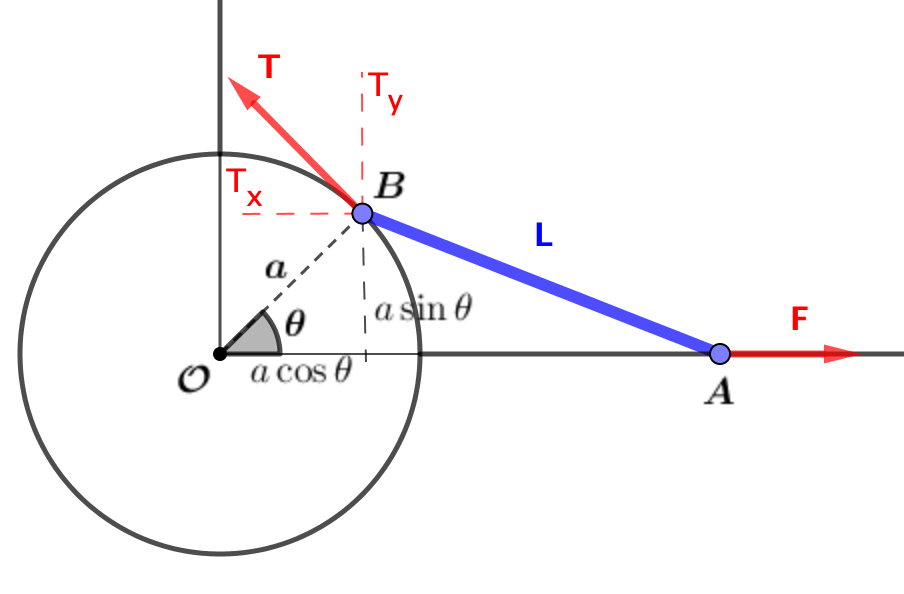
\includegraphics[width=.75\textwidth]{imagenes/imagenes06/T06IM10.png}
\end{figure}

$\vec F_A=F\ \vec i;\quad \vec F_B=-T\sin \theta \ \vec i + T\cos \theta \vec j$

$\vec r_A=[a\cos \theta +(L^2-a^2\sin^2 \theta)^{1/2}]\ \vec i; \quad \vec r_B=a\cos \theta \ \vec i + a \sin \theta \vec j$

$\var \vec r_A=[-a \sin \theta + \frac 1 2 (L^2-a^2 \sin^2 \theta)^{-1/2}\ 2 a^2 \sin\theta \cos \theta] \ \var \theta \ \vec i$

$\var \vec r_B=(-a \sin \theta \ \vec i+a\cos \theta \ \vec j)\ \var \theta$


Trabajos virtuales:  $\vec F_A \cdot \var \vec r_A+\vec F_B \cdot \var \vec r_B=0$


\small{$[-F a \sin \theta -F a^2 \sin \theta \cos \theta \ (L^2-a^2\sin^2 \theta)^{-1/2}\ + T a \sin^2 \theta + T a \cos^2 \theta]\ \cancelto{\neq 0}{\var \theta}=0 \to$}

\normalsize{$T=F\sin \theta \left( 1 + \dfrac{a \cos \theta}{(L^2-a^2\sin^2 \theta)^{1/2}} \right) \Rightarrow$}

$\dfrac T F = \sin \theta \left( 1+\dfrac {a \cos \theta}{(L^2-a^2\sin^2 \theta)^{1/2}}  \right) \ \to \ \ \ \theta=\pi/6 \ \Rightarrow \ \cdots$

\rightline{\textsf{\textcolor{DarkBlue}{--- Inacabado ---}}}




\begin{prob}
Un anillo está obligado a moverse en una elipse de 	semiejes $a$ y $b$. Sabiendo que el anillo pesa $P$ y que es solicitado por el eje $Y$ con una fuerza proporcional a la distancia a eje eje, determinar la posición de equilibrio.
\end{prob}
\begin{multicols}{2}
$\quad$

$ F_x=-Kx;\quad F_y=0 $

$P_x=0;\quad \quad \ \ P_y=-P$

$\quad$

$f : \ \dfrac{x^2}{a^2}+\dfrac{y^2}{b^2}=1$
\begin{figure}[H]
	\centering
	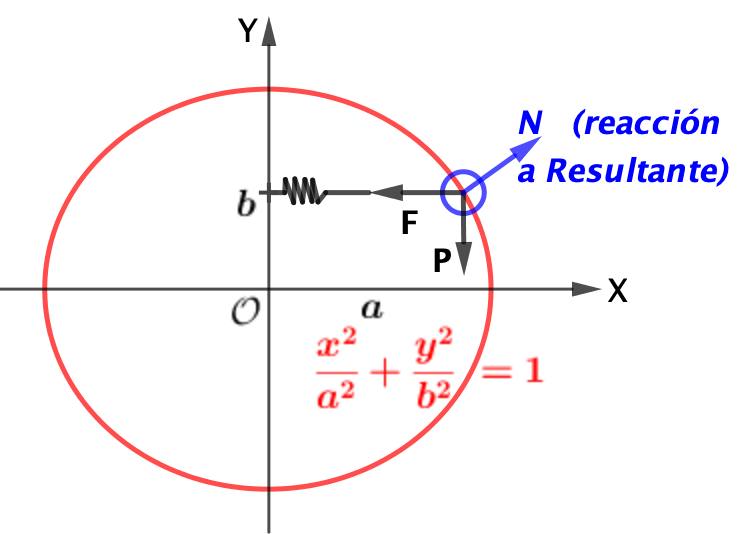
\includegraphics[width=.5\textwidth]{imagenes/imagenes06/T06IM11.png}
\end{figure}
\end{multicols}

$\left. \begin{matrix}  
 	\displaystyle N_x=\lambda \ \fdv{f}{x} \ \quad \\ \\ \displaystyle N_y=\lambda\  \fdv{f}{y} \ \quad 
 \end{matrix} \right|
 \left. \begin{matrix}  
 	\quad \lambda \ \displaystyle \fdv{f}{x}-Kx=0 \ \quad \\ \\ \quad \displaystyle \lambda \ \fdv{f}{y}-P=0 \quad 
 \end{matrix} \right|
\left. \begin{matrix}  
 	\quad \lambda \dfrac{2x}{a^2}-kx=0\ \quad (1*)\\ \\ \quad \lambda \dfrac{2y}{b^2}-P=0\  \quad (2*)
 \end{matrix} \right.$

$(1*)\ \to \ x\left(\dfrac{2\lambda}{a^2}-k \right)=0 \begin{cases}\ x=0 \to (f\to) \ y=\pm b \\ \ 2\lambda
=ka^2 \quad (3*) \end{cases}$

$(2*) \ \wedge \ (3*)\ \to \ y=\dfrac{Pb^2}{2\lambda}=\dfrac{Pb^2}{ka^2} \ \to f: \ x=\pm \dfrac 1{ka}\sqrt{k^2a^2-P^2b^2}$

Hay cuatro soluciones:

$(0,b);\ (0,-b);\ \left(\dfrac 1{ka}\sqrt{k^2a^2-P^2b^2},\dfrac{p^2b^2}{ka^2} \right);\ \left(-\dfrac 1{ka}\sqrt{k^2a^2-P^2b^2},\dfrac{p^2b^2}{ka^2} \right) $

\begin{prob}
	Una partícula de masa m se puede desplazar sin rozamiento siguiendo una parábola vertical $y=ax^2$, con a>0.
	
	Si en el punto $(0,H)$, con $H>0$, hay un centro de fuerzas que atrae a la partícula con una fuerza directamente proporcional a la distancia, ?`cuáles serán las posiciones de equilibrio de la partícula a lo largo de la parábola?
\end{prob}

\begin{multicols}{2}
$\sum F_x:\quad -Kx\ \vec i$

$\sum F_y:\quad -mg-k(y-H)\ \vec j$

$f:\quad y=ax^2 \quad (\var y= 2ax\ \var x)$

$\var \vec r_x=\var x\ \vec i;\quad \var \vec r_y=2ax\ \var x \ \vec j$

Trabajos virtuales:

$\vec F_x \cdot \var \vec r_x + \vec F_y \cdot \var \vec r_y=0$
\begin{figure}[H]
	\centering
	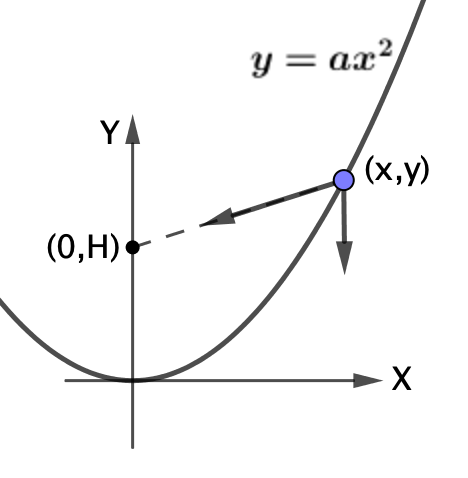
\includegraphics[width=.4\textwidth]{imagenes/imagenes06/T06IM12.png}
\end{figure}
\end{multicols}
$-kx \var x+ [-mg-k(y-H)]\ 2ax)\ \var v=0 \to \ (\var x \neq o)$

Despejando y teniendo en cuenta la relación entre $x$ e $y$ ($f:\ y=ax^2$), se obtienen las posiciones de equilibrio.

\rightline{\textsf{\textcolor{DarkBlue}{--- Inacabado ---}}}



\begin{comment}

% *******************************************************
% *** Dos problemas exámenes NO SEGURO e inacabados *****
% *******************************************************


\begin{multicols}{2}
\textbf{P.I. 4. } 

\textit{Una varilla de $6 \ \mathrm{kg}$ y longitud $0.8\ \mathrm{m}$ está colocada sobre un ángulo recto liso como muestra la figura adjunta. Determinar la posición de equilibrio y las fuerzas de reacción en función del ángulo $\theta$}.
\begin{figure}[H]
	\centering
	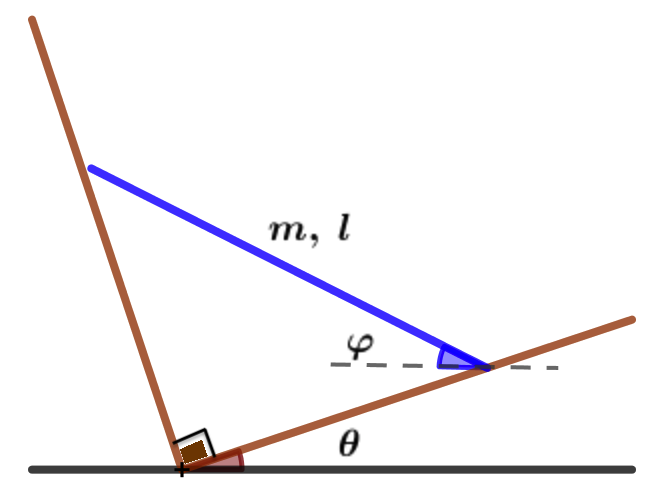
\includegraphics[width=.45\textwidth]{imagenes/imagenes09/T09IM13.png}
\end{figure}
\end{multicols}

$m=6 \ \mathrm{kg};\quad l=0.8\ \mathrm{m}; \qquad \to \qquad \boldsymbol{ N_1 (\theta), \ N_2 (\theta) , \ \varphi (\theta) }$

\begin{figure}[H]
	\centering
	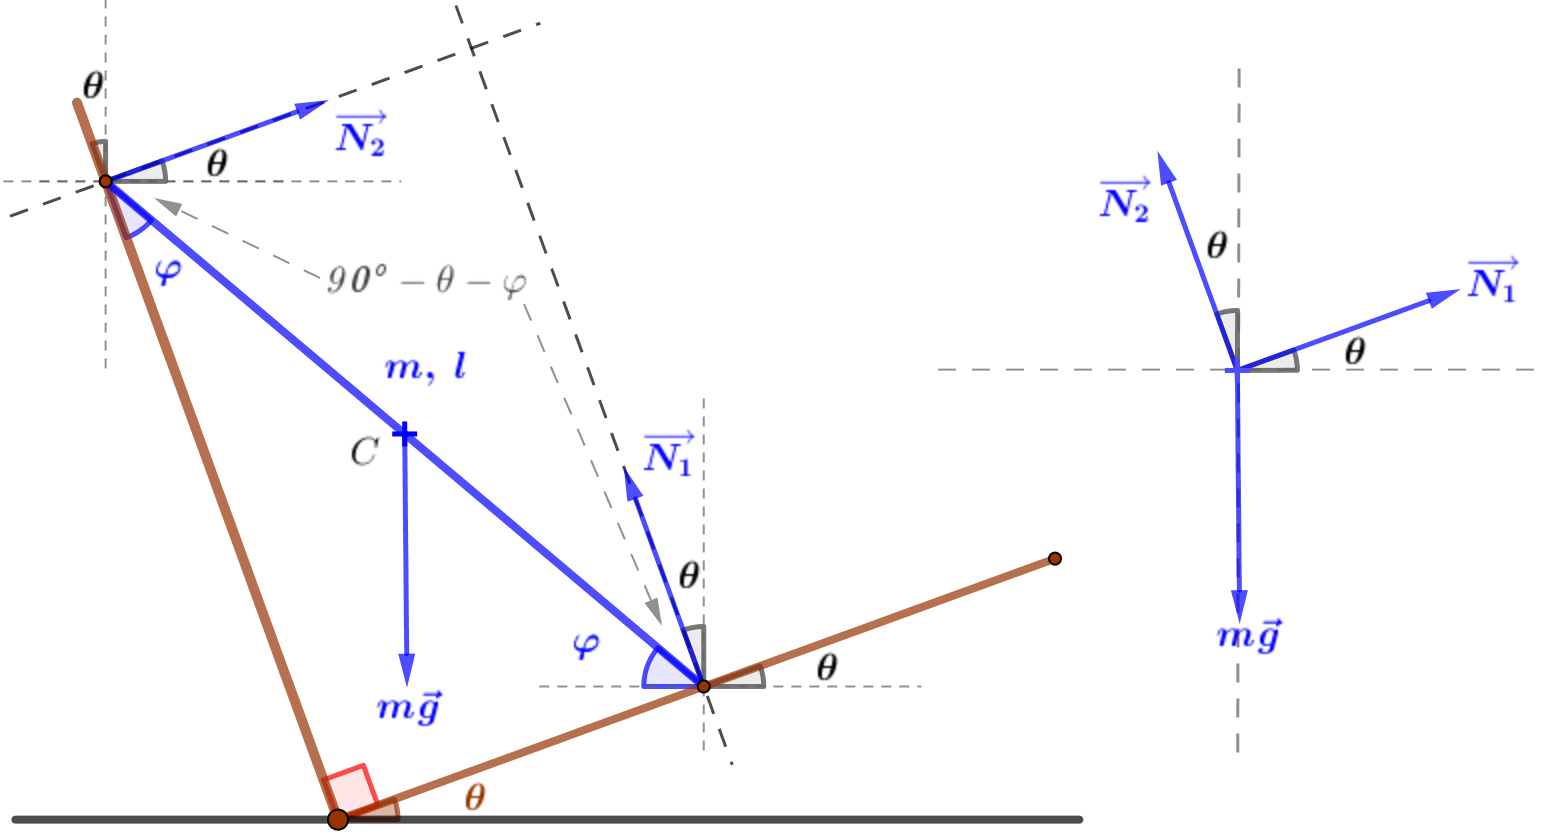
\includegraphics[width=1\textwidth]{imagenes/imagenes09/T09IM12.png}
\end{figure}

$\displaystyle \sum F_x=0: \qquad \boldsymbol{N_2 \cos \theta-N_1 \sin \theta = 0}$


$\displaystyle \sum F_y=0: \qquad  \boldsymbol{N_2 \sin \theta + N_1 \cos \theta - m g=0}$

Tomamos el origen de momentos en el punto $C$, centro de gravedad de la barra.

$\displaystyle \sum M_z=0: \ mg\cdot 0+ N_1 \dfrac L 2 \sin(90^ o-\theta-\varphi)-N_2\dfrac L 2 \sin(90^ o-\theta-\varphi)=0 \to $

$\displaystyle \boldsymbol{\dfrac {N_1L} 2 \cos (\theta-\varphi) - \dfrac {N_2L} 2 \cos (\theta-\varphi)=0}$

Incógnitas $N_1,\ N_2, \ \varphi; \qquad \text{datos: }\ m,\ l,\theta $

\rightline{\textsf{\textcolor{DarkBlue}{--- Inacabado ---}}}


\begin{multicols}{2}
\textbf{P.I. 5. } \textit{Dos partículas de masas $m_1$ y $m_2$ están situadas una sobre un plano inclinado de ángulo $\alpha$ y longitud $L$ y la otra sobre un punto de cuarto de aro de radior $R$ y unidas entre sí por un hilo inextensible de longitul $l$ y masa despreciable.}
\begin{figure}[H]
	\centering
	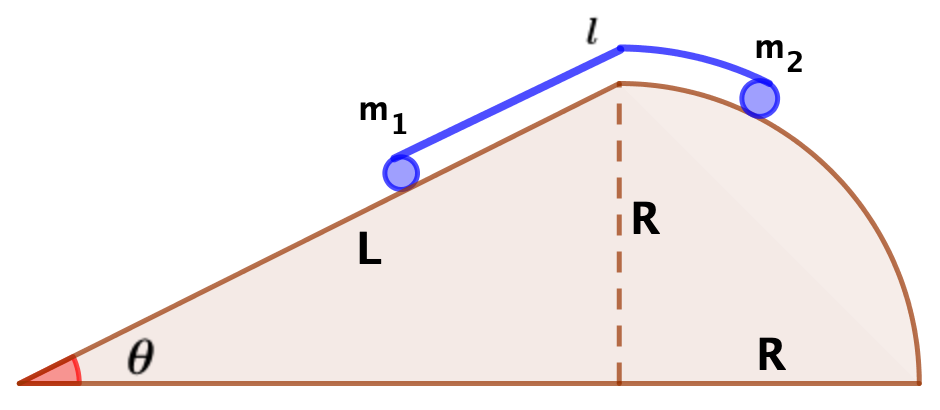
\includegraphics[width=.5\textwidth]{imagenes/imagenes09/T09IM14.png}
\end{figure}
\end{multicols}

\textit{Si tanto la superficie del aro como la del plano son lisas, determinar cuál es la posición de equilibrio. Como particularización, calcular la posición de equilibrio para $m_1=m_2=1\ \mathrm{kg},\ \alpha=30^o \text{ y } L=l=1\ \mathrm{m}$}


Datos: $\quad m_1=m_2=1\ \mathrm{kg},\ \alpha=30^o \text{ y } L=l=1\ \mathrm{m}$

Incógnitas: $\quad \boldsymbol{N_1, \ N_2,\; x \text{ ó } \varphi}$

\begin{figure}[H]
	\centering
	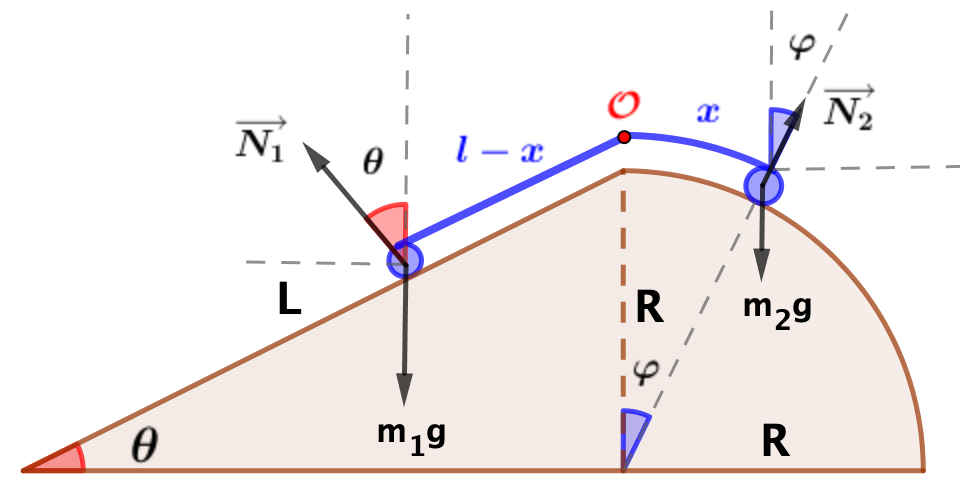
\includegraphics[width=.75\textwidth]{imagenes/imagenes09/T09IM15.png}
\end{figure}

arco=ángulo (rad) x radio $\ \to x=\varphi R \ \to \boldsymbol{\varphi=\dfrac x R }$

$\displaystyle \sum F_y:\quad (m_1+m_2)g-N_1\cos \theta-N_2 \cos \phi$

$\displaystyle \sum F_x:\quad -N_1\sin \theta + N_2 \sin \varphi=0$

Tomamos como centro de momentos el punto $\ \mathcal O$:

$\displaystyle \sum M:\ \  -N_1 (l-x)+m_1g(l-x)\sin(\frac \pi 2 - \theta)+N_2x-m_2gx \sin (\dfrac \pi 2 - \varphi)=0$

$\boxed{ \  \begin{cases}
\ N_1\sin \theta-N_2\sin \varphi=0 \\
\ N_1\cos \theta+N_2\cos \varphi=(m_1+m_2)g \\
\ (m_1g\cos \theta - N_1)\ (l-x)=(m_2g\cos \varphi-N_2)\ x
\end{cases} \ }$

Incógnitas $N_1, \ N_2, \ \varphi$; datos: $m_1,\ m_2,\ \theta, R, l$

Relación $x,\ l:\quad \varphi=x R;\quad \sin \theta=\dfrac R L$

\rightline{\textsf{\textcolor{DarkBlue}{--- Inacabado ---\textit{\footnotesize{principio trabajos virtuales???}\normalsize{---}}}}}

$N_1,\ N_2\ \bot \ \var r \to W=m_1g\cos (\frac \pi 2 - \theta)-m_2g \cos (\frac \pi 2 - \varphi) \ \var r=0 \to $

$m_1g\sin \theta =m_2g\sin \varphi \to \sin \varphi =\dfrac {m_1}{m_2}\sin \theta $

\rightline{\textsf{\textcolor{DarkBlue}{--- Tan fácil ???? ---}}}


Y si pruebo a calcular la energía potencial y exijo que sea mínima

\rightline{\textsf{\textcolor{DarkBlue}{--- Probarlo!!!!!! ---}}}

\begin{figure}[H]
	\centering
	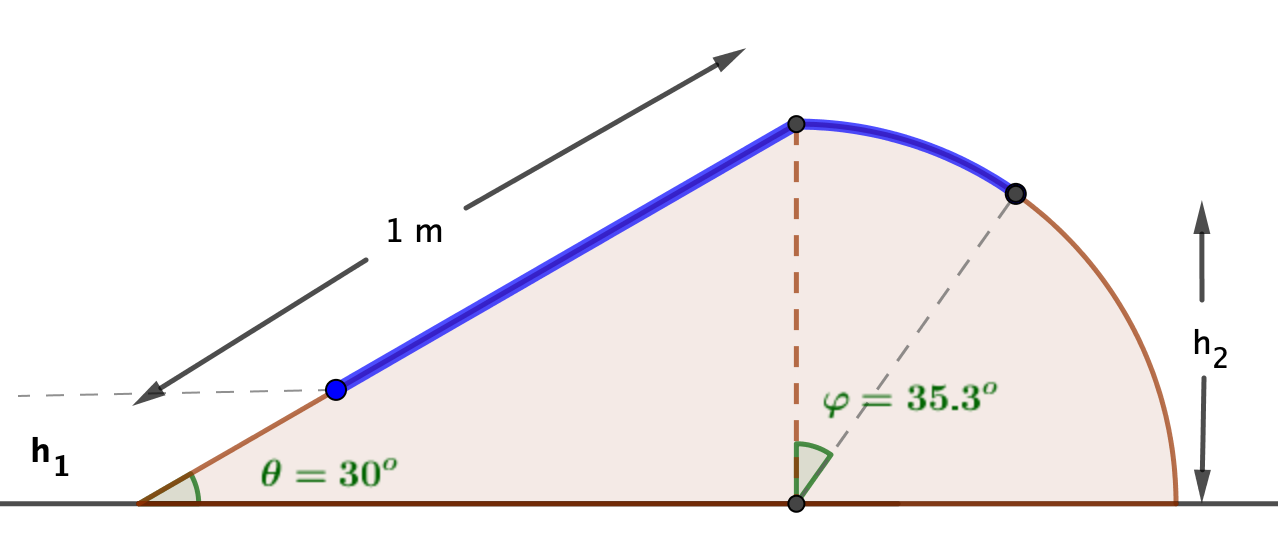
\includegraphics[width=.75\textwidth]{imagenes/imagenes09/T09IM16.png}
\end{figure}

$E_p=m_1gh_1+m_2gh_2$

$h_1=(l-x) \sin \theta; \qquad x=\varphi L \sin \theta:\quad \varphi=\dfrac{x}{L\sin \theta}$

$h=2=R\cos \varphi=L \sin \theta \cos \varphi = L \sin \theta \cos \left( \dfrac{x}{L\sin \theta} \right)=E_p(x)$

$\displaystyle \dv{E_p}{x}=0 \to -m_1g\sin \theta \textcolor{red}{+} m_2gL\sin \theta \dfrac {1}{L \sin \theta} \sin \left( \dfrac{x}{L\sin \theta} \right)=0$

$\sin \left( \dfrac{x}{L\sin \theta} \right)= \dfrac{m_1}{m_2}\tan \theta$

Datos: $ \dfrac{x}{1/2}=\arcsin \left( \dfrac{\sqrt{3}}{3} \right) \to x=0.308\ \mathrm{m};\quad l-x=0.616\ \mathrm{m};\quad \varphi=0.161 \ \mathrm{rad}=35.29^o$
 
\textcolor{red}{Debería ser un MENOS}

\rightline{\textsf{\textcolor{DarkBlue}{--- Probar dos cuerpos separados, T, ....!!!!!! ---}}}

	
\end{comment}



\begin{prob}
\begin{multicols}{2}.
Una varilla de longitud $2L$ y peso $P$ está en equilibrios en el borde y en la superficie de una cápsula hemiesférica de radio $R<L$, sin rozamiento. 

Determinar la posición de equilibrio.	
\begin{figure}[H]
	\centering
	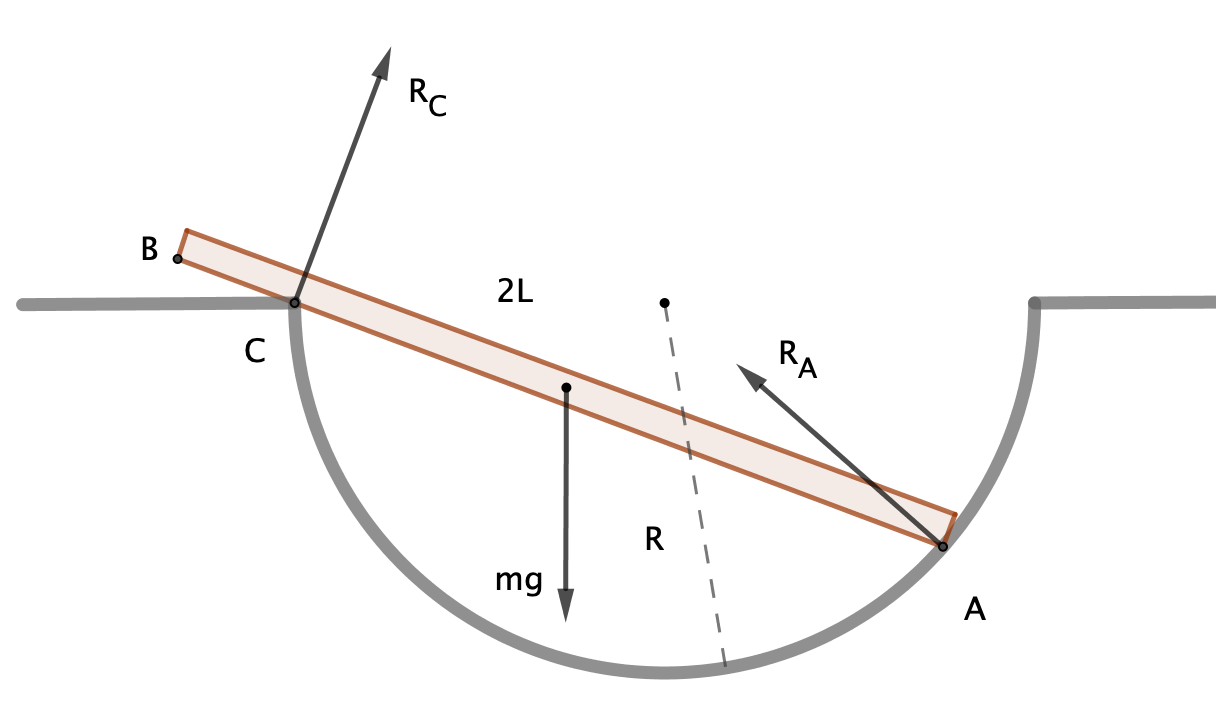
\includegraphics[width=.55\textwidth]{imagenes/imagenes06/T06IM13.png}
\end{figure}
\end{multicols}	
\end{prob} 

La posición de equilibrio viene determinada por el ángulo $\boldsymbol{\theta}$, como se muestra en la siguiente figura en que se han dibujado las fuerzas que actúan y se han elegido los ejes $x$ e $y$ como allí se indica. Exigiremos que $\sum F_x=0$, $\sum F_y=0$ y $\sum M_z=0$. Escogemos como centro de momentos el punto $A$, con lo anulamos el de la reacción $R_A$.

\begin{figure}[H]
	\centering
	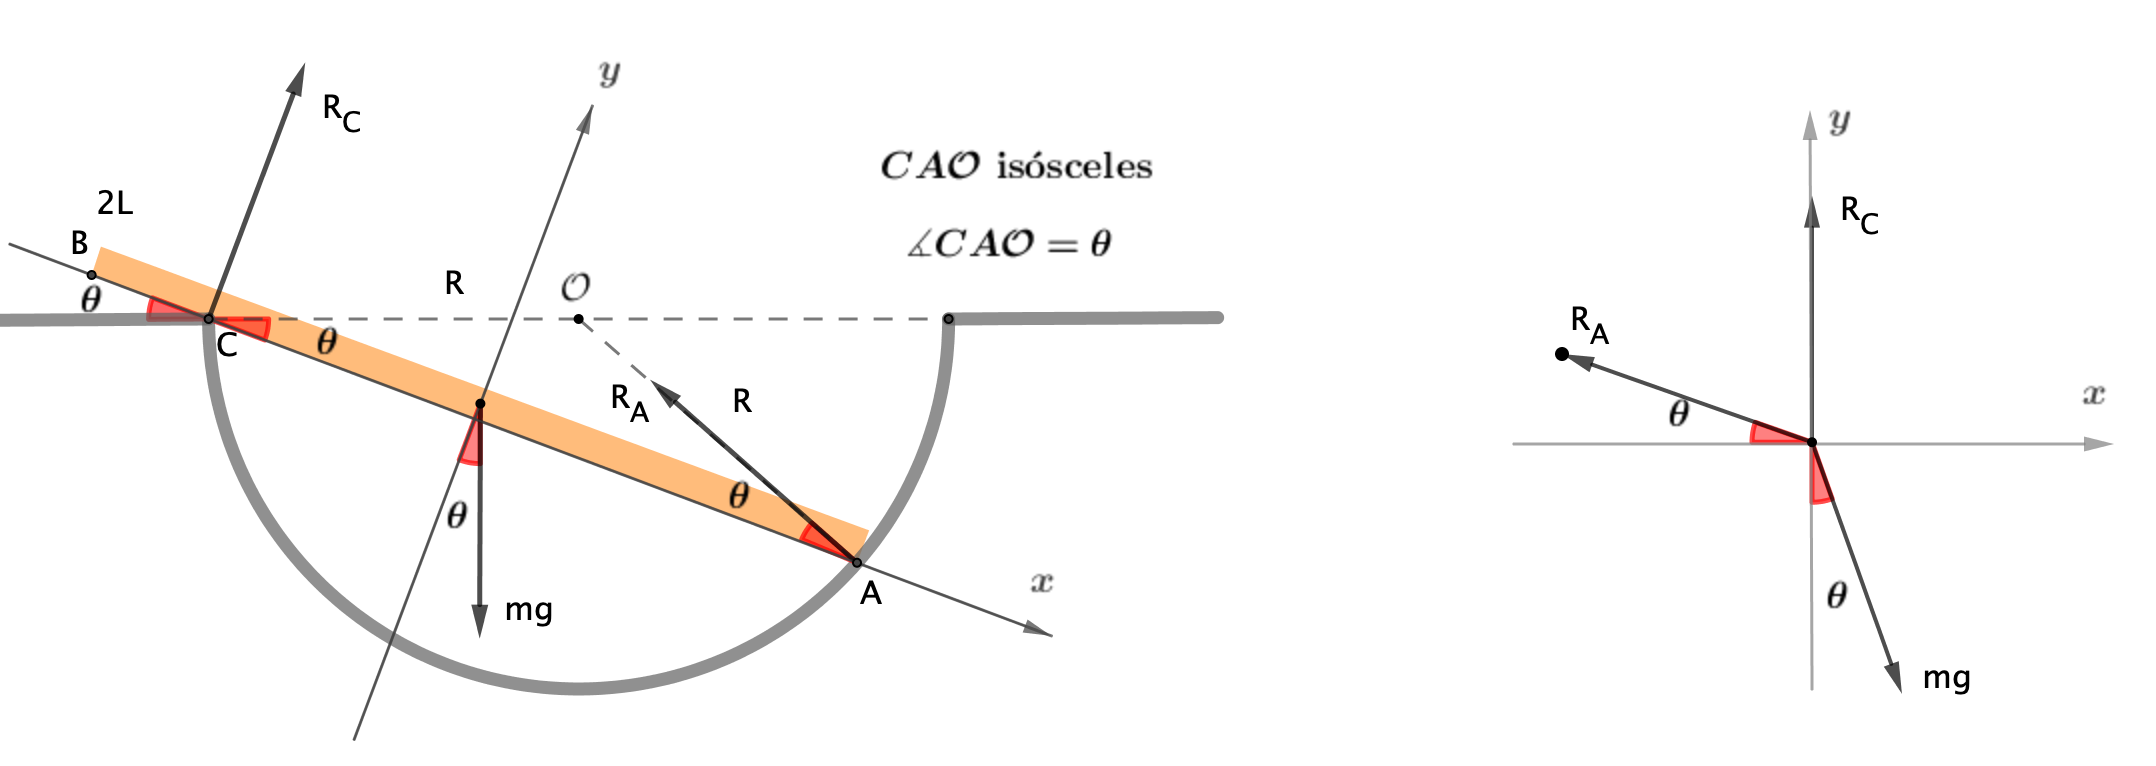
\includegraphics[width=1.1\textwidth]{imagenes/imagenes06/T06IM14.png}
\end{figure}

$\sum F_x=0 \ \to \ -R_A \cos \theta + P \sin \theta =0 \quad \textcolor{gris}{(1*)}$

$\sum F_y=0 \ \to \ R_C-P\cos \theta+R_A \sin \theta=0 \quad \textcolor{gris}{(2*)}$

$\sum M_z=0 \ \to \ -R_C \overline{AC} + PL \cancelto{\cos \theta}{\sin(90^o-\theta)}=0 \quad \textcolor{gris}{(3*)}$

De la figura, $\ \dfrac{\overline{AC}}{2}=R \cos \theta \ \to \ \overline{AC}=2R\cos \theta \quad \textcolor{gris}{(4*)}$

De $\textcolor{gris}{(1*)} \ \to \ -R_a+P\tan \theta = 0;\qquad \boldsymbol{R_A=P \tan \theta}$

De $\textcolor{gris}{(3) \text{ y } (4*)} \ \to \ -R_c 2R \cos \theta + PL \cos \theta = 0;$

$ \cos \theta \cdot \left( -2R_cR+PL \right) =0; \quad \cos \theta \neq 0 \quad  \to \ \boldsymbol{R_C=\dfrac{PL}{2R}}$

Llevándolo a $\textcolor{gris}{(2*)} \ \to \ \dfrac {PL}{2R} - P \cos \theta + P \tan \theta \sin \theta = 0$

$P\cdot \left( \dfrac {PL}{2R} - \cos \theta +  \tan \theta \sin \theta \right) = 0; \quad  P\neq 0 \ \to$

$\dfrac {L}{2R} - \cos \theta +  \tan \theta \sin \theta = 0 $

$ \tan \theta \sin \theta = \dfrac{\sin^2 \theta}{\cos \theta}$, multiplicando por $\cos \theta$ la ecuación anterior,

 $\dfrac {L}{2R} \cos \theta - \cos^2 \theta + 1- \sin^2 \theta =0 \ \to \ -2\cos^2 \theta + \dfrac L{2R} \cos \theta + 1 = 0$
 
 $\boldsymbol{\cos \theta=} \dfrac{-\dfrac{l}{2R} \pm \sqrt{\left(\dfrac{L}{2R}\right)^2 + 8} }{-4}=\cdots =\boldsymbol{
 \dfrac L {8R} + \sqrt{\left( \dfrac{l}{8R} \right)^2 + \dfrac 1 2} }$


\begin{prob}.
	Una barra uniforme de masa $M$ y longitud $L$ se sos	tiene es sus extremos por medio de una cuña como se muestra en la figura. Encontrar las reacciones normales en los puntos de apoyo y el ángulo de equilibrio.
\end{prob}

\begin{figure}[H]
	\centering
	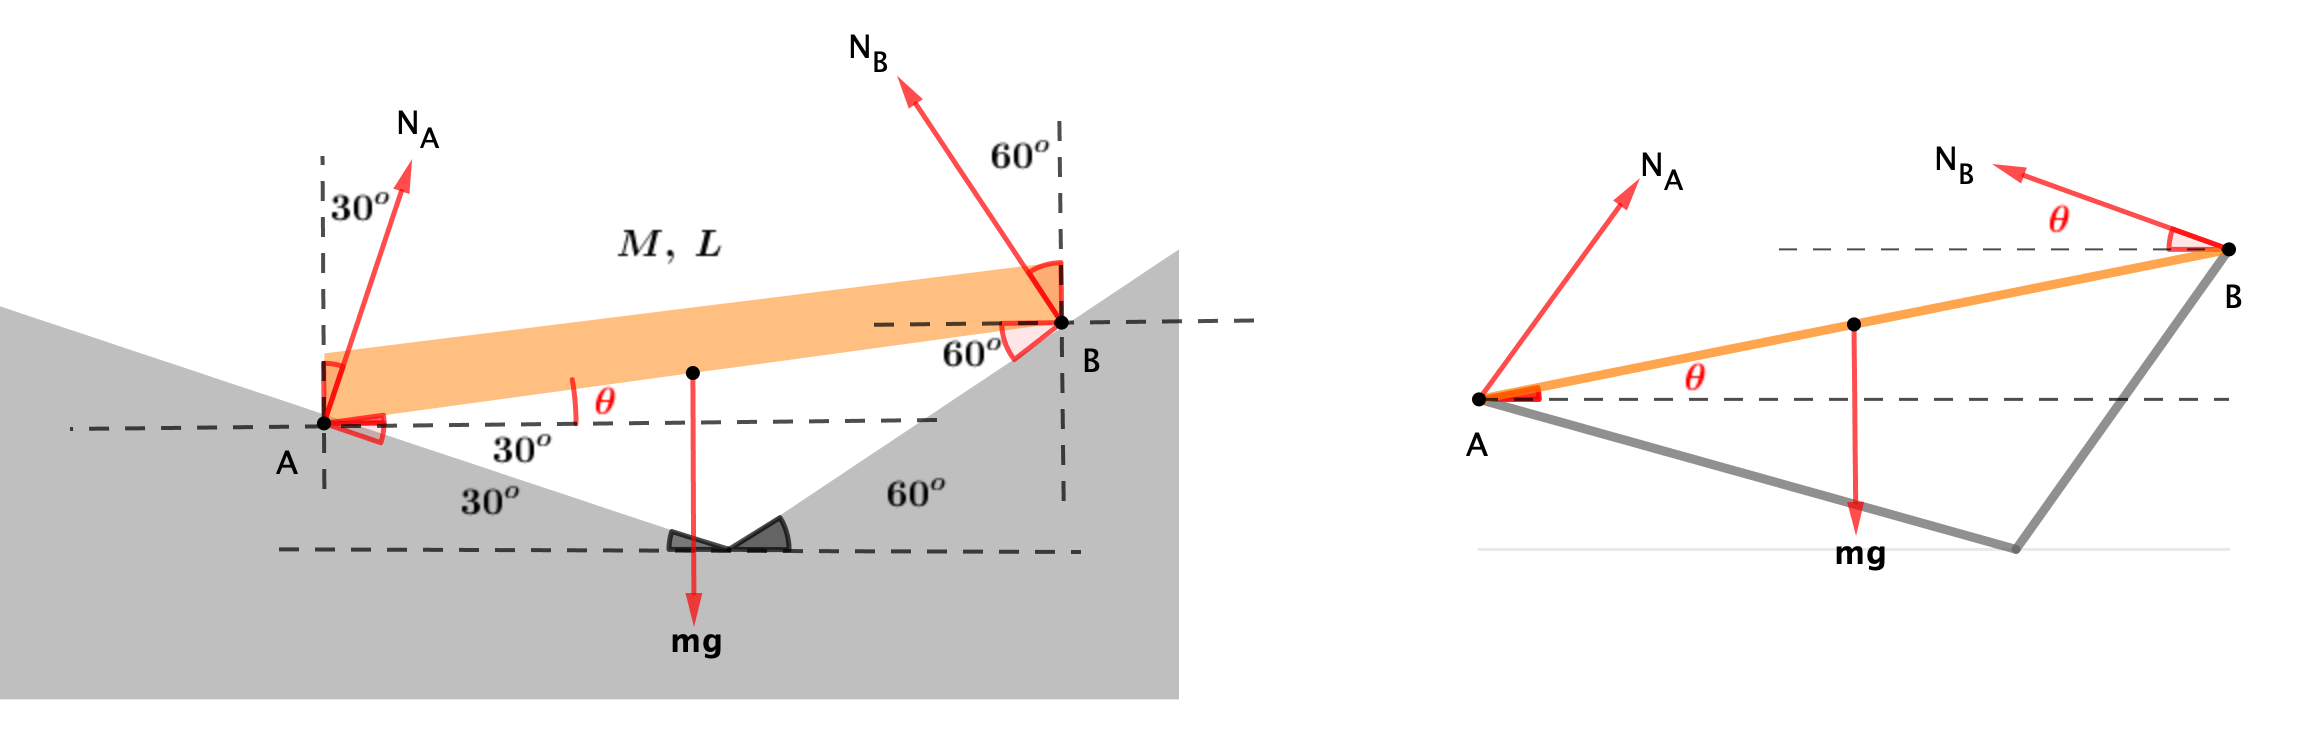
\includegraphics[width=1\textwidth]{imagenes/imagenes06/T06IM17.png}
\end{figure}

$\sum F_x=0:\quad N_A\sin30^o-N_B\sin 60^0=0 \quad \to \quad N_B=N_A\tan 30^o \ \textcolor{gris}{(*)}$

$\sum F_y=0:\quad N_A \cos 30^o+ N_B \cos 60^o - mg = 0 \quad \to $

$N_A \cos 30^0 + N_A \tan 30^0 \sin 30^0 =mg;\quad N_A(\cos^2 30ô + \sin^2 30^o)=mg \cos 30^0$

$ \boldsymbol{N_A=mg\cos 30^0}$

$\textcolor{gris}{(*)}\ \to \quad \boldsymbol{N_B=}mg\cos 30^o \tan 30^o =\boldsymbol{mg \sin 30^o}$

Tomamos el origen de momentos es $A$, así anulamos uno de ellos (el de $N_A$).

$\sum M_z=0:\quad N_a\cdot 0 +mgr_C-NB\sin \theta r_B=0;\quad mg\dfrac L 2 \cos(\theta-30^o)-mg \cancelto{1/2}{\sin 30^o} \sin \theta L = 0$

$mg\dfrac L 2 \cos (\theta-30^o)=mgL \dfrac 1 2 \sin \theta \quad \to \quad \cos(\theta-30^o) = \sin \theta$

Como $\cos \alpha=\sin (90-\alpha) \quad \to \quad \cos(\theta-30^o)=\cos(90^o-\theta)$,

por lo que: $\ \theta-30^o=90^o - \theta \quad \to \quad \boldsymbol{\theta= 60^o}$



\newpage %*******************************

\begin{myblock}{El Principio de los Trabajos Virtuales.}
Principio de los trabajos virtuales.

\vspace{2mm} El Principio de Trabajos Virtuales fue utilizado por Galileo (1564-1642) para el diseño y c cálculo de mecanismos y desarrollado teóricamente con un enunciado más matemático y formal por Lagrange (1736-1813. 

\vspace{2mm} El núcleo teórico del Pincipio  de los Trabajos Virtuales fue enunciado por Santiago Bernouilli (1654-1705) y por Daniel Bernouilli (1700-1782): “Si una estructura, estando en equilibrio, sufre una deformación virtual debido a la acción de una carga adicional , el trabajo virtual externo de la carga en cuestión, es igual al trabajo virtual interno, desarrollado por las tensiones causadas por la carga”. 

\vspace{2mm} En cuanto a lo que concierne a la mecánica de cuerpos rígidos, dado que por definición estos cuerpos no sufren deformación sino desplazamientos, el Pincipio  de los Trabajos Virtuales debe ser reformulado. El mismo fue enunciado por Johann Bernouilli en el año 1717 de la siguiente manera: “Dado un cuerpo rígido mantenido en equilibrio por un sistema de fuerzas, el trabajo virtual efectuado por este sistema, durante un desplazamiento virtual, es nulo”. 
\end{myblock}


